\documentclass[tikz,border=1mm]{standalone} 
\usetikzlibrary{positioning,shadows,shapes.symbols,shapes.geometric}

% colors
\definecolor{myblue}{rgb}{0.4, 0.6, 0.8}
\definecolor{mycoral}{rgb}{0.97,0.51,0.47}
\definecolor{mygreen}{rgb}{0.66,0.89,0.63}
\definecolor{myocra}{rgb}{1, 0.8, 0.4}
\definecolor{mypurple}{rgb}{0.7, 0.6, 0.9}

\renewcommand{\familydefault}{\sfdefault}

\begin{document}

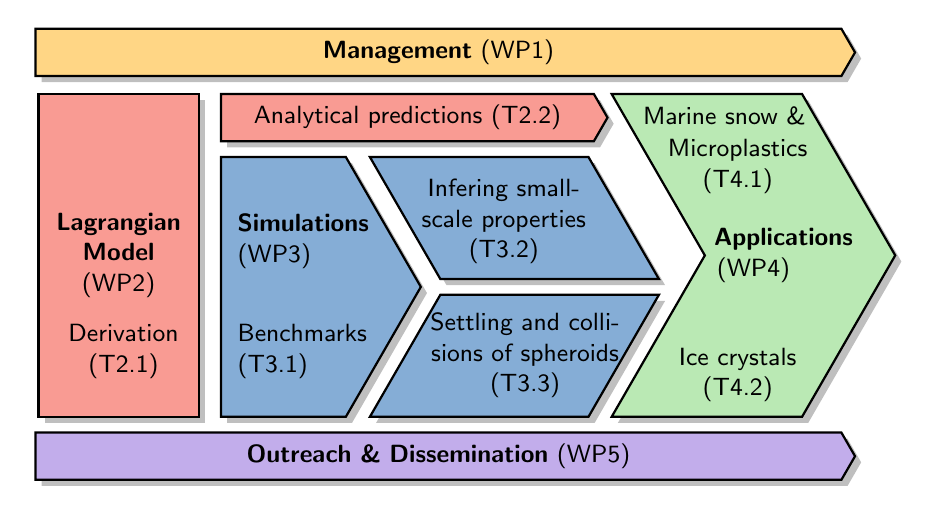
\begin{tikzpicture}[font=\small]

% Management WP1
\node[signal, thick, drop shadow, signal pointer angle=120, align=center, text width=10cm, minimum height=0.6cm, draw=black, fill=myocra!80] 
(wp1) {{\bf Management} (WP1)};

% Dissemination WP5
\node[signal, thick, drop shadow, signal pointer angle=120, align=center, text width=10cm, minimum height=0.6cm, draw=black, fill=mypurple!80, below=4.5cm of wp1] 
(wp5) {{\bf Outreach \& Dissemination} (WP5)};

% Lagrangian Model WP2
\node[thick, drop shadow, align=center, text width=1.8cm, minimum height=4.1cm, fill=mycoral!80, draw=black, below left=2mm and -2.1cm of wp1] 
(desc) {{\bf Lagrangian Model}\\ (WP2)};

% Toy models WP2
\node[signal, thick, drop shadow, signal pointer angle=120, align=center, text width=4.5cm, minimum height=0.6cm, fill=mycoral!80, draw=black, below right=2mm and -7.9cm of wp1] 
(pred) {Analytical predictions (T2.2)};

% DNS Benchmarks WP3
\node[signal, thick, drop shadow, signal pointer angle=120, align=left, text width=1.35cm, minimum height=3.3cm, fill=myblue!80, draw=black, below right=10.mm and -7.9cm of wp1] 
(dns0) {};
\node at (-1.55,-2.4)[align=left, text width=2cm] {{\bf Simulations}\\ (WP3)};
\node at (-1.55,-3.8)[align=left, text width=2cm] {Benchmarks\\(T3.1)};

% DNS with neutral spheroids WP3
% Infering small-scale properties of stratified turbulence from spheroid orientation
\node[trapezium, trapezium left angle=120, trapezium right angle=60, thick, drop shadow, align=left, text width=0.05cm, minimum height=1.55cm, fill=myblue!80, draw=black, below right=10.mm and -4.95cm of wp1] 
(dns1) {};
%\node at (0.83,-2.15)[align=center, text width=2.5cm] {Neutrally buoyant\\ Spheroids\\ (T3.2)};
\node at (0.83,-2.15)[align=center, text width=2.5cm] {Infering small-scale properties\\ (T3.2)};


% DNS with settling spheroids WP3
\node[trapezium, trapezium left angle=60, trapezium right angle=120, thick, drop shadow, align=left, text width=0.05cm, minimum height=1.55cm, fill=myblue!80, draw=black, below right=27.5mm and -4.95cm of wp1] 
(dns2) {};
\node at (1.1,-3.85)[align=center, text width=3cm] {Settling and collisions of spheroids\\ (T3.3)};
%{Settling Spheroids\\ (T3.3)};

% Applications WP4
\node[signal, thick, drop shadow, signal pointer angle=120, text width=1.0cm, align=center, minimum height=4.1cm, fill=mygreen!80, draw=black, below right=2mm and -2.95cm of wp1, signal from=west] 
(wp4) {{\bf Applications}\\ (WP4)};
\node at (3.7,-0.8)[align=left, text width=2.2cm] {Marine snow \&};
\node at (3.8,-1.45)[align=center, text width=2cm] {Microplastics\\(T4.1)};
\node at (3.8,-4.1)[align=center, text width=2cm] {Ice crystals\\(T4.2)};

% other writings
\node at (-4.0,-3.8)[align=center, text width=2.2cm]  {Derivation\\(T2.1)};

\end{tikzpicture}

\end{document}